\newSec[HWCOEX]{COEX Drohne}{2}

Bei dem für die \DHBW\ neu angeschafften \Quad\ handelt es sich um das Modell \Clover\ des Unternehmens \textit{Copter Express} (\COEX).

Das \Quad-Familie \textit{Clover} wurde vom Hersteller zur Ausbildung und Forschung an \Quad[n] entwickelt. Das Modell besitzt einen Rahmen, welche die Rotoren bei Kollisionen schützten soll.




Interner Flight Controller, ROS Kommunikation via Pie 4.




Probleme bei Inbetriebnahme - Beispielprogramm des Herstellers bringt nicht das erwartete Ergebnis.




\newSec[Control]{Control Stack}{3}
Als \textit{Flight Controller} wird das Modell \textit{PX4 Racer} genutzt. Die Firmware, sowie weitere Software zur Interaktion mit der Drohne \Clover\ werden von \textit{Dronecode Foundation} bereitgestellt.

Die Anbindung an \ROS wird durch einen \Pie\ realisiert. Hierbei wird der On-Board Computer als \textit{roscore} genutzt.


\newSec{Sensorik}{3}
\begin{itemize}
\item Gyroskop
\item Laser-Abstandsmessung zum Boden
\item GPS
\item Bodenkamera
\end{itemize}


\newSec[Build]{Aufbau des Bausatzes}{3}
\newSec{Aufbau}{4}
Der Aufbau und die Verkabelung des \Quad[s] \Clover\ wurden entsprechend der Hersteller-Vorgaben (siehe \cite{coexAssembly}) durchgeführt.

\begin{figure}[ht!]
\vspace{0.25cm}
\begin{center}
\fbox{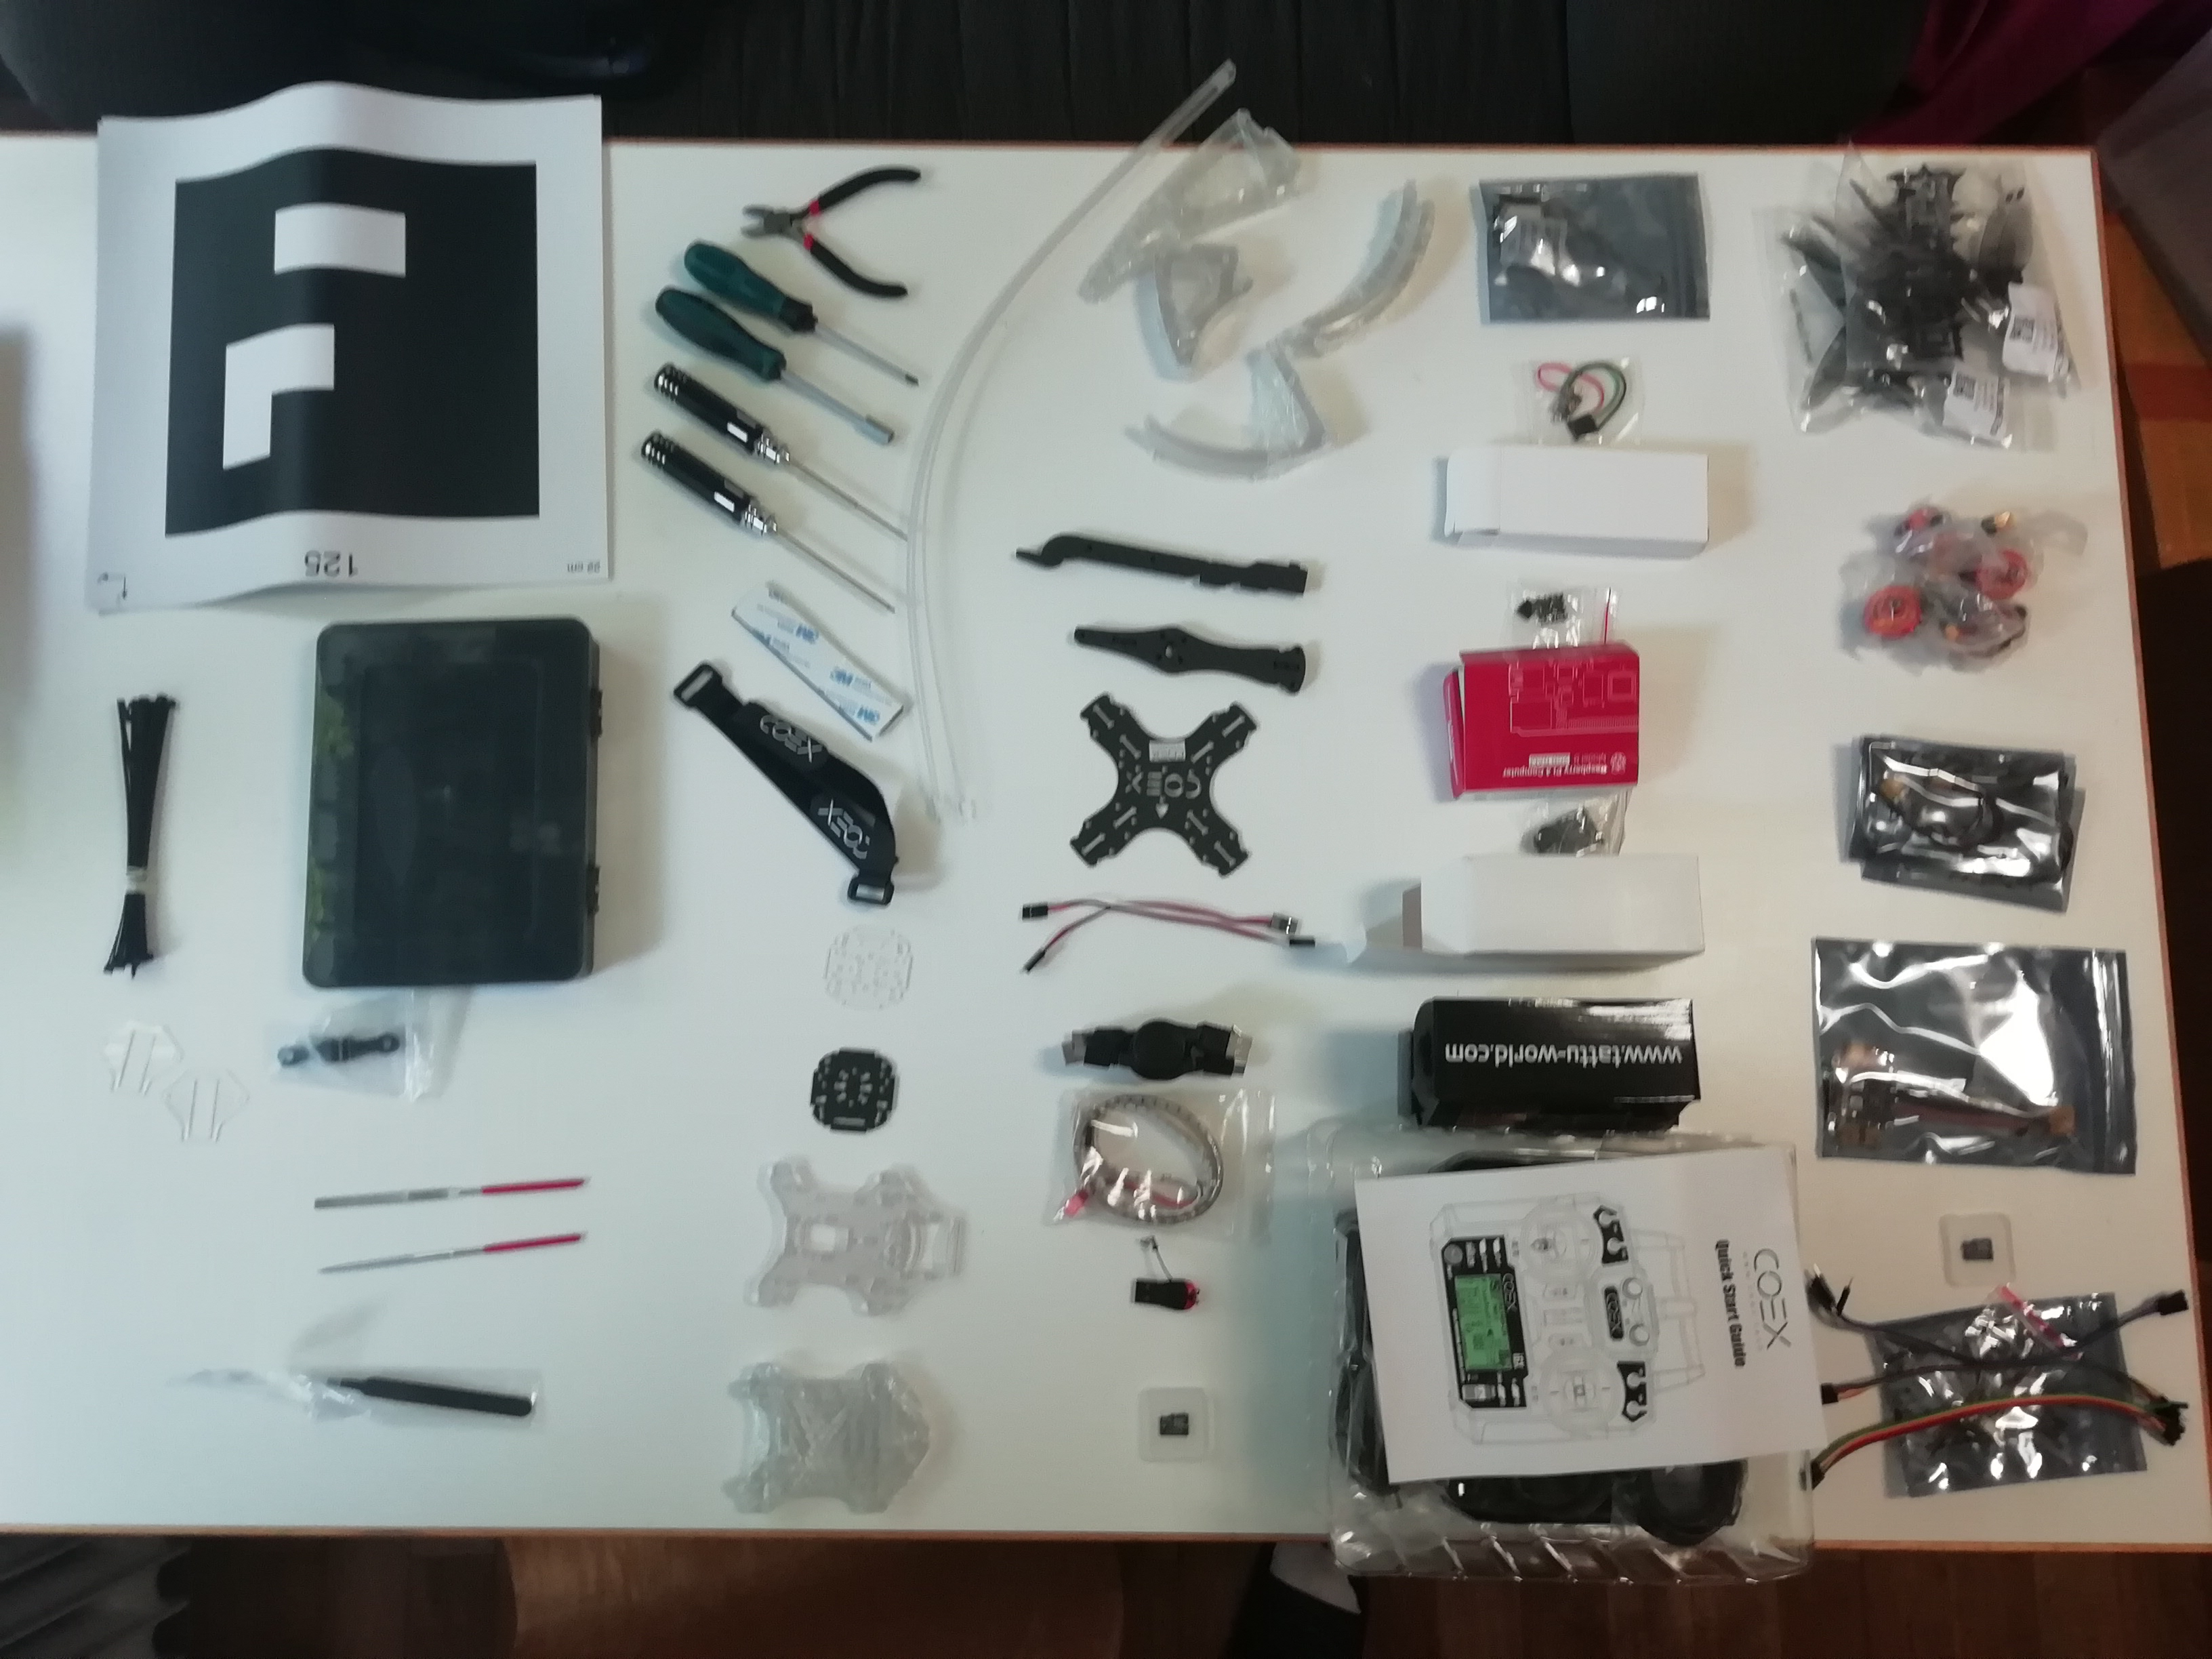
\includegraphics[width=7.5cm]{Pictures/Aufbau1.jpg}}\hfill
\fbox{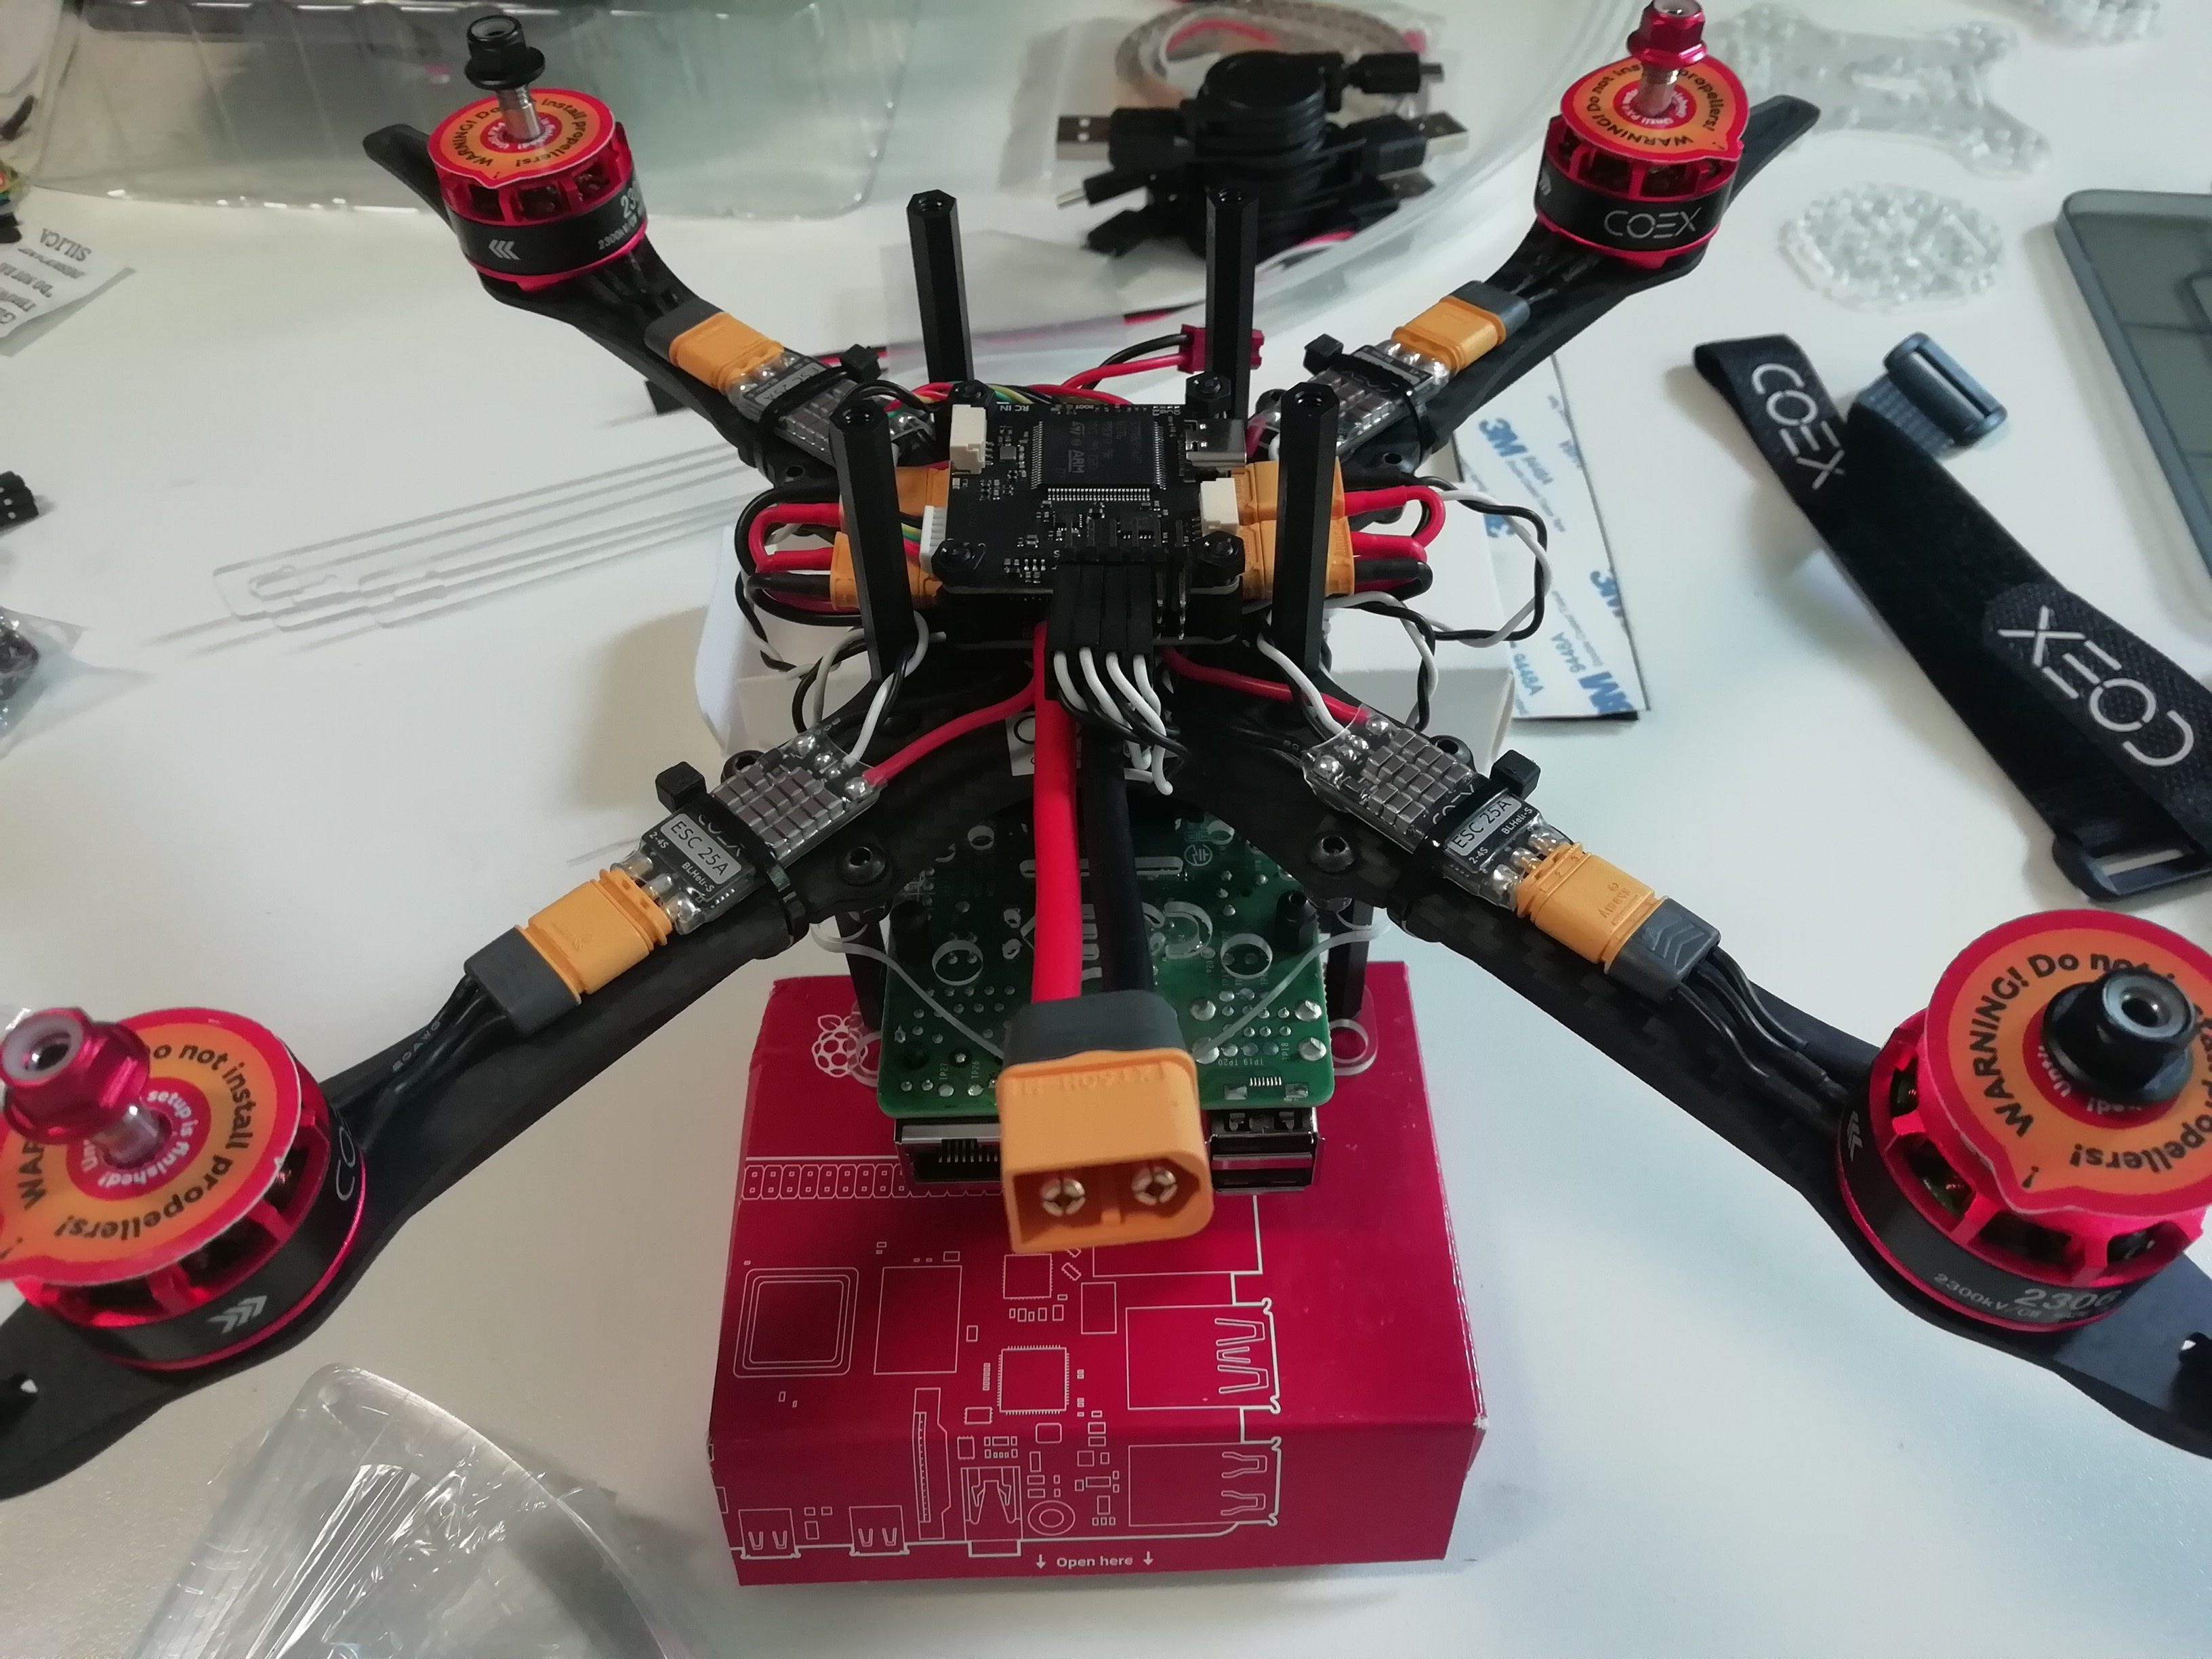
\includegraphics[width=7.5cm]{Pictures/Aufbau2.jpg}}
\fbox{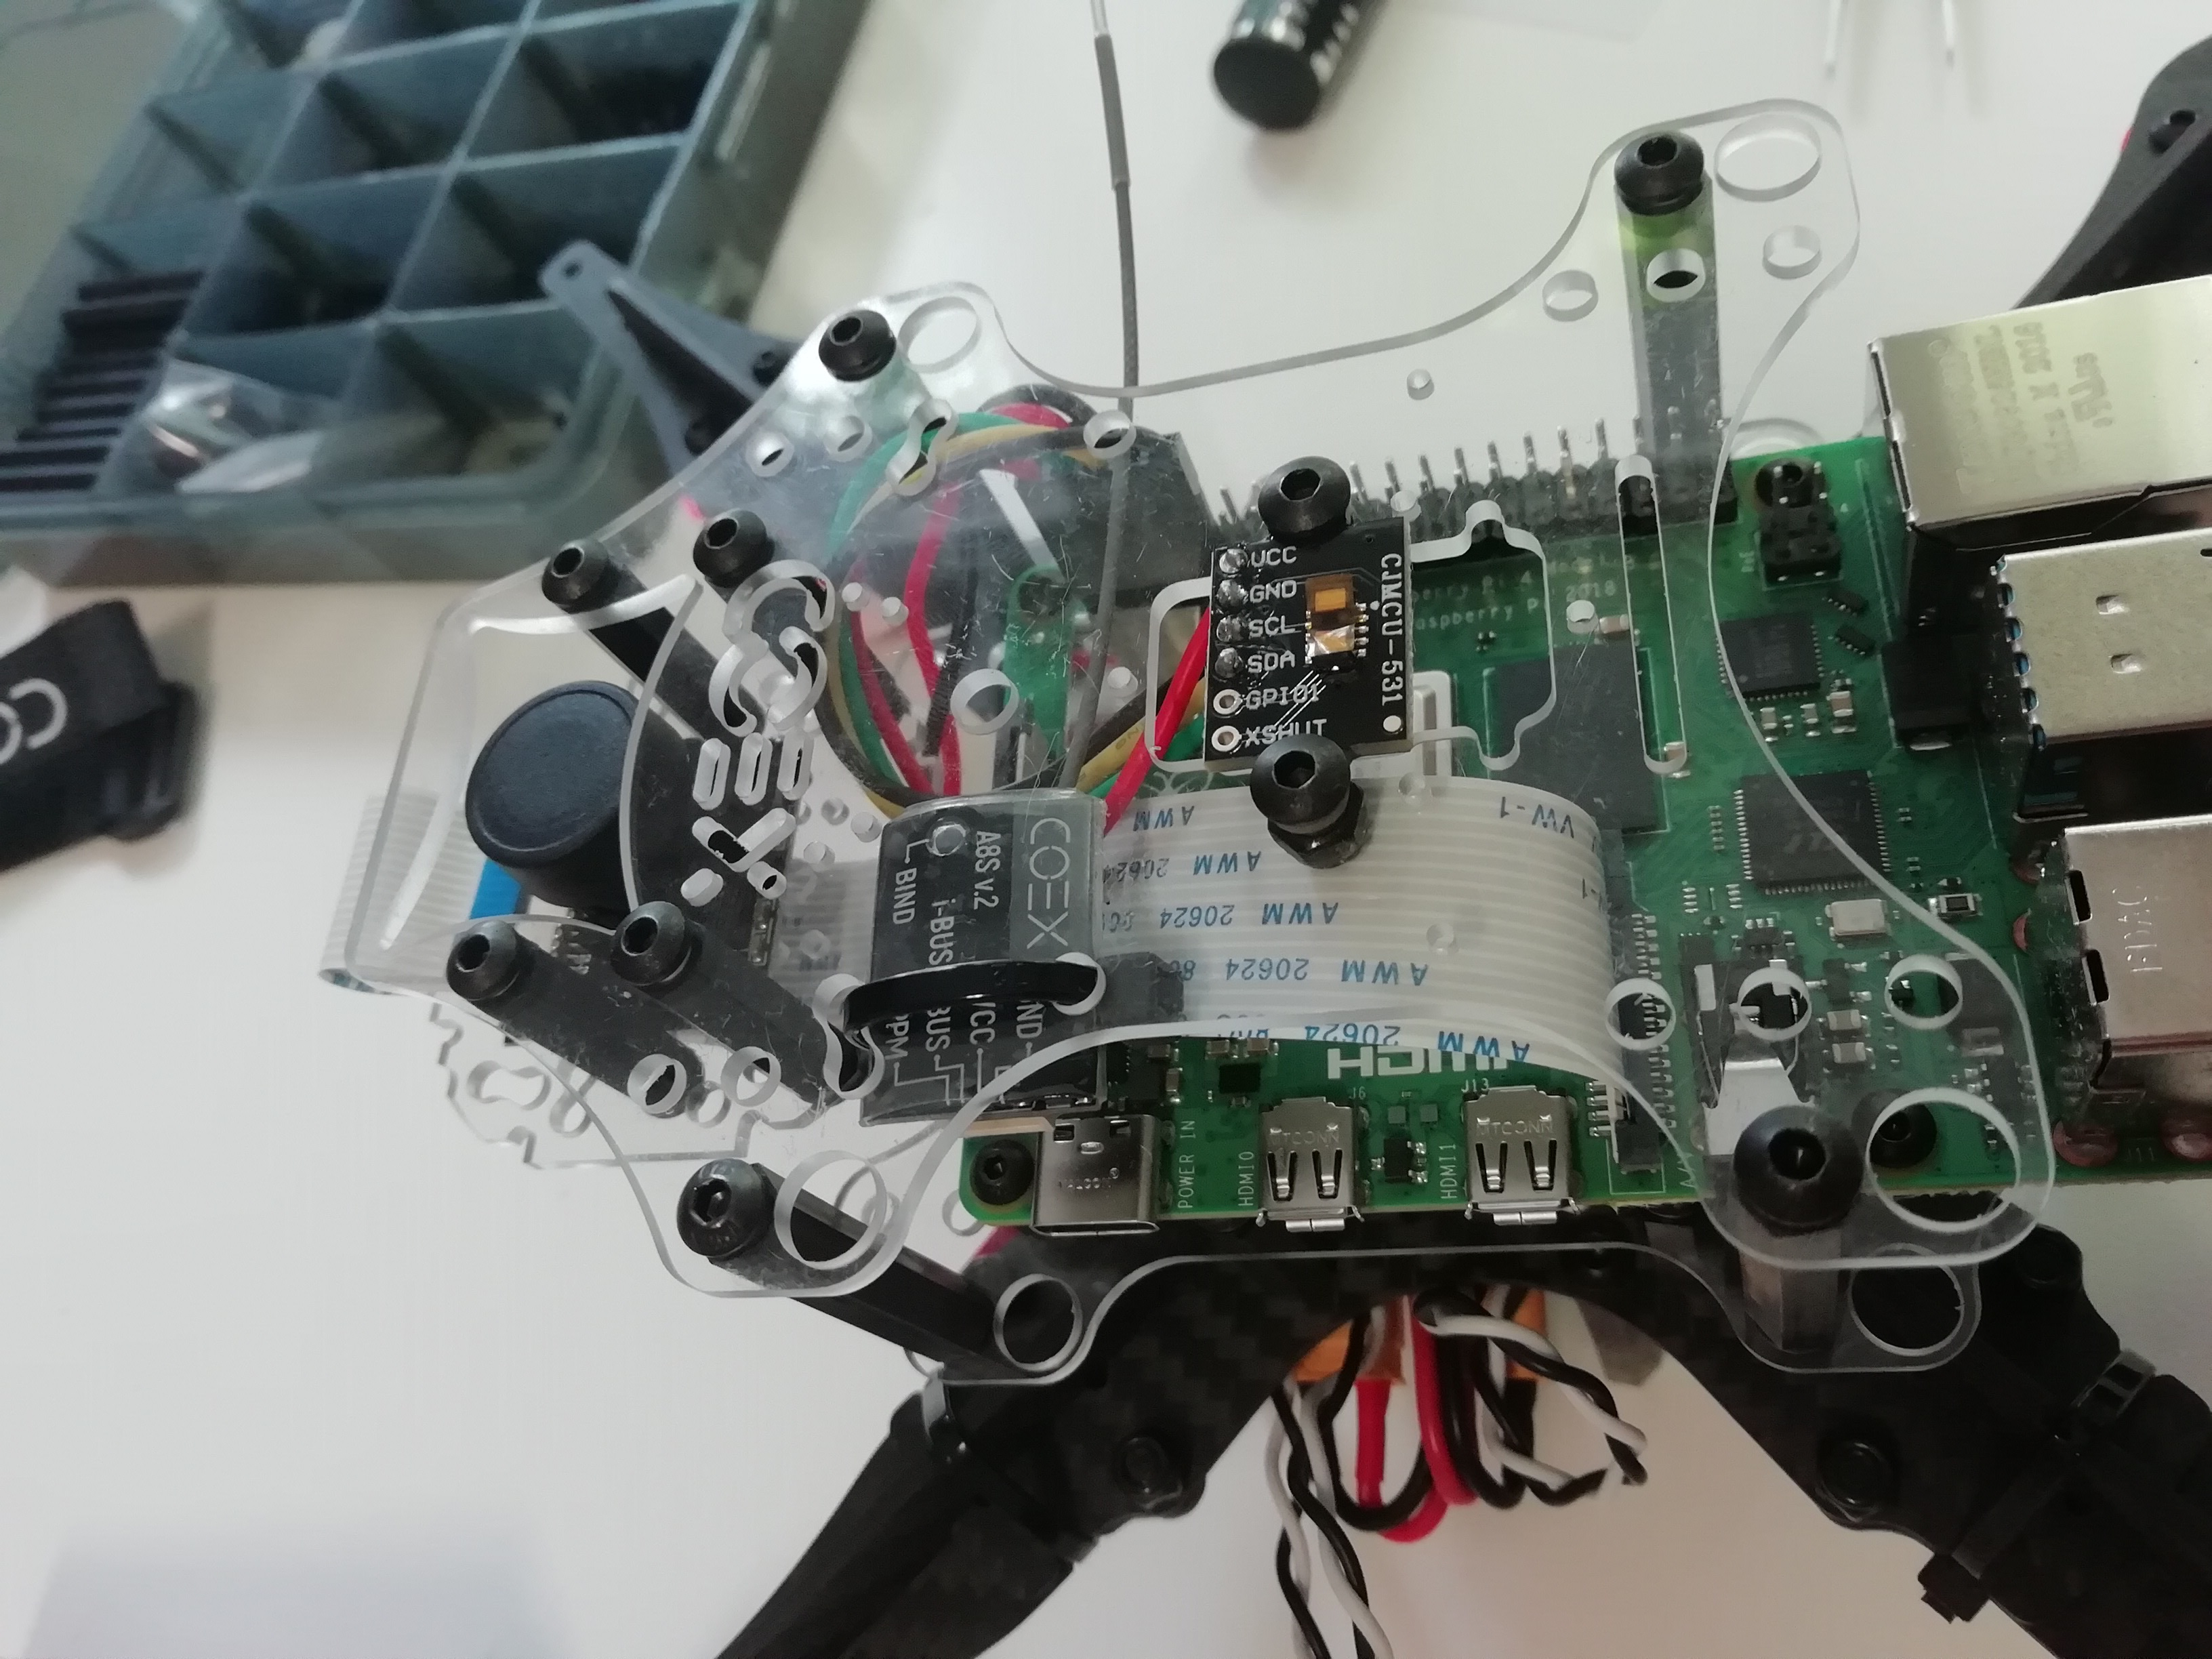
\includegraphics[width=7.5cm]{Pictures/Aufbau3.jpg}}\hfill
\fbox{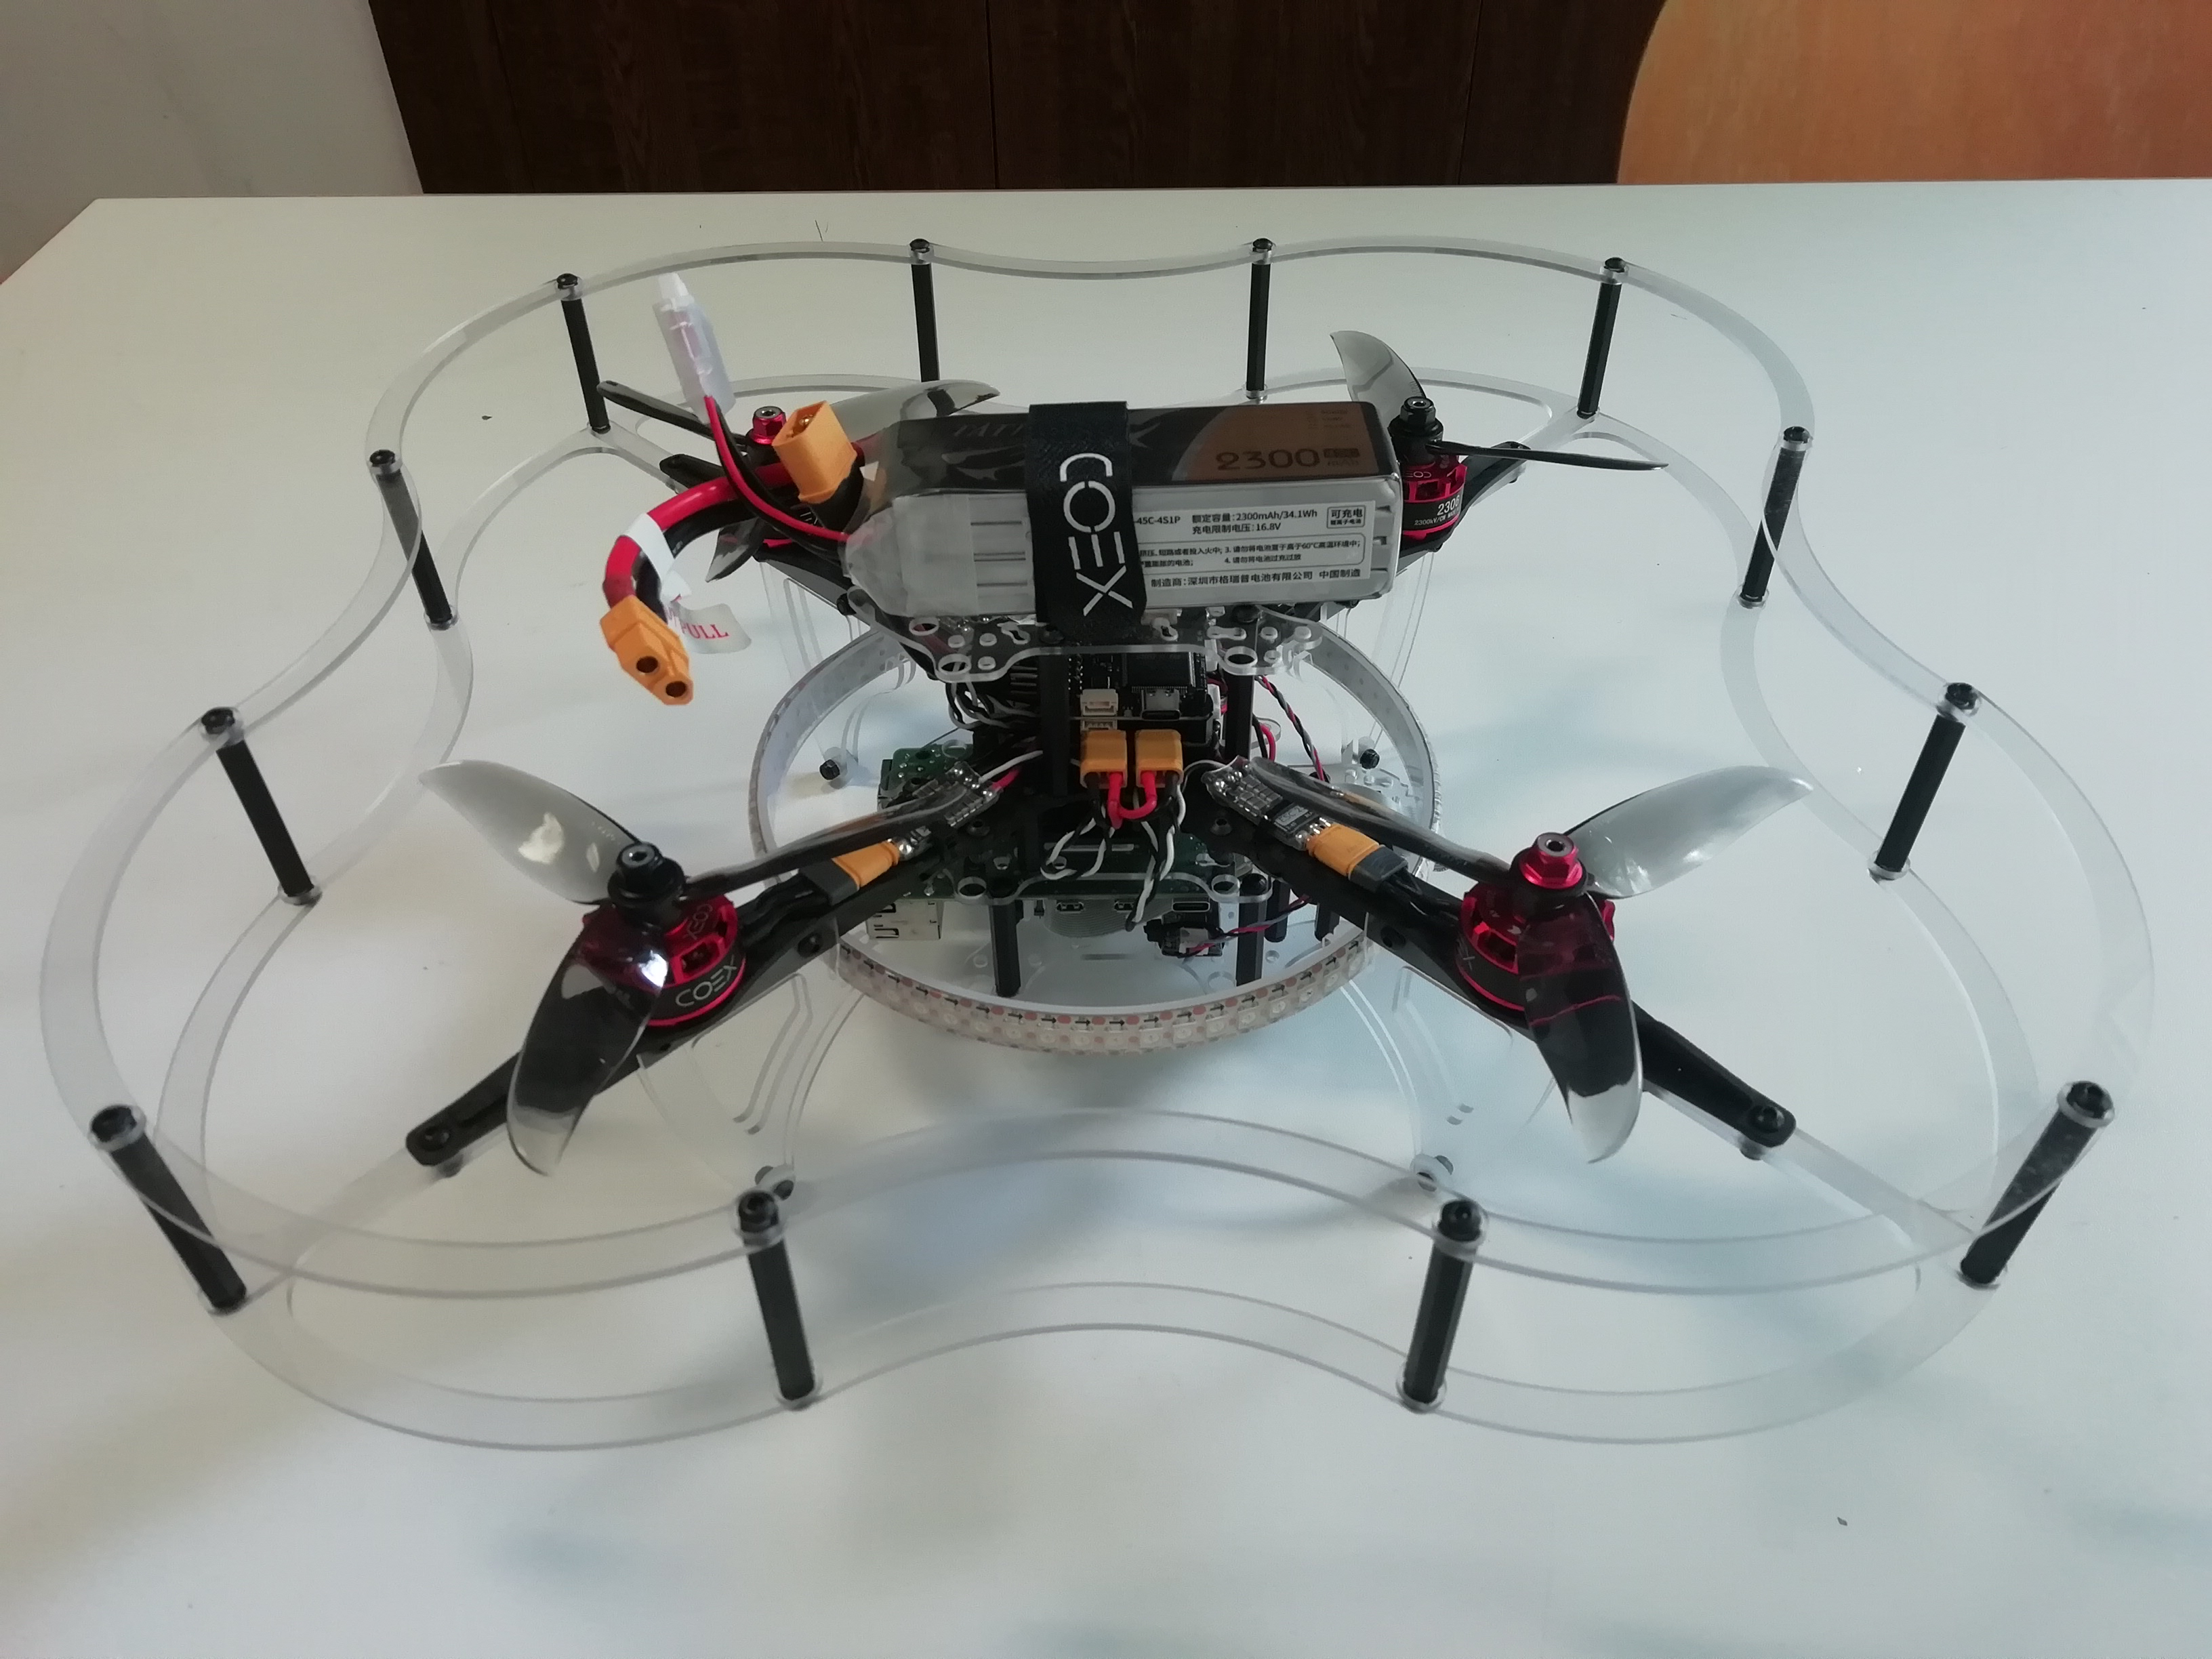
\includegraphics[width=7.5cm]{Pictures/Aufbau4.jpg}}
\caption{Aufbau des Bausatzes für die Drohne \Clover}
\label{fig:coexBuild}
\end{center}

\vspace{0.25cm}
\refImgShort{fig:coexBuild} zeigt etappenweise den Aufbau des Bausatzes für die Drohne \Clover. Hierbei ist die zeitliche Anordnung in der Collage zeilenweise zu interpretieren.
\end{figure}


\newSec[FireUp]{Inbetriebnahme}{3}
\newSec{Konfiguration des Flight Controllers}{4}
Die Konfiguration wurde entsprechend der Hersteller-Empfehlung mittels die Software \textit{QGroundControl} durchgeführt. Sämtliche Anweisungen der Hersteller-Vorgaben (siehe \cite{coexConfig}) wurden befolgt.\\
Das für den \textit{Flight Controller} aufgespielte Image entspricht der Version v0.22.


\newSec{Testflug}{4}
Nach einer vollständigen Konfiguration des \Clover\ wurde ein Beispielprogramm zum Testen des \Quad[s] genutzt. Dieses Programm wird vom Hersteller des \textit{Flight Controller} zur Verfügung gestellt \cite{coexExample}.\\
Das Programm sieht vor, den \Quad\ nach dem Start auf einer Höhe von 2 m in einem Hover-Modus zu halten. Um die Sicherheit dieses Versuches zu erhöhen, wurde die Flughöhe dieses Testflugs reduziert. Im Verlauf des Testfluges zeigte sich, dass die vorgegebene Höhe nicht gehalten wurde. Der \Quad\ wurde durch eine baulichen Begrenzung davon abgehalten, weiter an Höhe zu gewinnen.\\
Eine Rekalibrierung der Sensorik konnte diesem Umstand nicht entgegenwirken. Der Ansatz, diverse andere Topics zur Steuerung des \Clover\ einzusetzen, schlug ebenfalls fehl.\footnote{Eine Auswahl an Herangehensweisen ist im Git-Repository im Ordner \href{https://github.com/MobMonRob/ROSLabDrohne/tree/evolveSignalProcessing/Code/Text\_coex/src}{Text\_coex} hinterlegt.} Der Austausch der Hardware hin zu einem bewährten \Quad\ wurde durch diese Flugversuche mit dem \Quad\ \Clover\ hervorgerufen.


\newSec[Build]{Mögliche Lösung der Aufgabenstellung}{3}
\newSec[COEXPkg]{COEX-Package}{4}
Für die Interaktion mit der \COEX-Drohne wurden diverse Klassen erstellt, um einzelne Aspekte der Interaktion mit der Drohne umsetzen zu können (siehe \refCap{ImplPlugCOEX}).

Nach dem Wechsel auf die andere Drohne wurde die Aktualisierung dieses Package nicht weiter verfolgt. Sofern eine Einbindung der \COEX-Drohne in die Ergebnisse dieser \Arbeit\ durchgeführt werden soll, müss dieses Package entsprechend angepasst werden.


\newSec[COEXPkgTopic]{geeignete Topics}{4}
Mit dem \rTopic{setpoint\_raw/local} kann eine Regelung in der XY-Ebene umgesetzt werden. Die Höhenregelung kann mit dem \rTopic{set\_attitude/thrust} eingeführt werden.
Die Umsetzung mit den genannten \Topic[s] entspricht der Lösung der Aufgabenstellung entsprechend \refCap{Problemstellung}.

Alternativ zu der genannten Lösung können Stellgrößen als Befehle der Funkfernsteuerung immitiert werden. Das \rTopic{/mavros/rc/override} erlaubt das Überschreiben der RC-Kanäle, somit können die Eingaben durch den Regelkreis übernommen werden. Eingaben Nutzender sind durch eine entsprechend implementierte Daten-Brücke weiterhin möglich.


\newSec[CoexLiteratur]{hilfreiche Literatur}{4}
Nachfolgend sollen Internetseiten genannt werden, welche die Einarbeitung in den Umgang mit der \COEX-Drohne vereinfachen können.

\begin{itemize}
\item \href{https://clover.coex.tech/en/wifi.html}{https://clover.coex.tech/en/wifi.html}
\item \href{https://clover.coex.tech/en/simple\_offboard.html}{https://clover.coex.tech/en/simple\_offboard.html}
\item \href{https://docs.px4.io/master/en/ros/mavros\_offboard.html}{https://docs.px4.io/master/en/ros/mavros\_offboard.html}
\item \href{https://docs.px4.io/master/en/flight\_modes/offboard.html}{https://docs.px4.io/master/en/flight\_modes/offboard.html}
\item \href{https://mavlink.io/en/services/manual\_control.html}{https://mavlink.io/en/services/manual\_control.html}
\item \href{http://wiki.ros.org/mavros\#mavros.2FPlugins.manual\_control}{http://wiki.ros.org/mavros\#mavros.2FPlugins.manual\_control}
\item \href{https://mavlink.io/en/messages/common.html\#SET\_POSITION\_TARGET\_LOCAL\_NED}{https://mavlink.io/en/messages/common.html\#SET\_POSITION\_TARGET\_LOCAL\_NED}
\end{itemize}

Spezifische Verweise sind im Quellcode des \COEX-Package hinterlegt.



\newSec[COEXTrouble]{Troubleshooting}{3}
\newSec{Platinenfehler}{4}
Es zeigte sich nach Messungen, dass die Spannungsversorgung des LED-Streifens verpolt an die entsprechende Platine angebracht wurde.
Als Folge wird der Verpolungsschutz des LED-Streifns aktiv, wodurch die Spannung aller Komponenten des \textit{Control Stack} auf etwa 0.6V abfällt.\\
Der LED-Streifen zählt nicht zu des essentiellen Bauteilen des \Quad. Der \Quad\ kann ohne die Nutzung des LED-Streifens betrieben werden.


\newSec{Bus-System des RC Empfängers}{4}
Der RC-Empfänger gibt die Funk-Signale über einen Bus an den \textit{Flight Controller} weiter. Hierbei ist zu berücksichtigen, dass der RC-Empfänger die beiden  Bus-Protokolle \textit{i-Bus} und \textit{s-Bus} versenden kann. Der Inhalt beider Protokolle ist identisch. Der Unterschied besteht in der Signal-Invertierung.\\
\begin{tabbing}
\hspace{3.5cm} \= \kill
RC-Sender:\>\href{https://www.flysky-cn.com/i6-gaishu}{FS-i6}\\
RC-Empfänger:\>\href{https://www.flysky-cn.com/x8b-canshu}{FS-X8B}
\end{tabbing}

\texttt{Lösung}\\
\textit{BIND}-Knopf beim Einschalten für etwa 3 Sekunden gedrückt halten. Der Bus-Mode wird hiermit umgeschalten.


\newSec[TopicTroubleRCOverMD5]{md5-Sum des Topics OverrideRCIn}{4}
Nach erfolgreicher Kompilierung wird nachfolgender Laufzeitfehler ausgegeben, wenn sich eine Instanz der \CodeClass{ros::Subscriber} oder der \CodeClass{ros::Publisher} auf das \rTopic{/mavros/rc/override} anmeldet:\\
\textcolor{red}{[ERROR] [1643616625.226584828]: Client [/mavros] wants topic /mavros/rc/override \\to have datatype/md5sum [mavros\_msgs/OverrideRCIn/73b27a463a40a3eda1f9fbb1fc86d6f3], but our version has [mavros\_msgs/OverrideRCIn/fd1e1c08fa504ec32737c41f45223398]. Dropping connection.}

\texttt{Lösung}\\
Definition von \\\CodeStruct{struct MD5Sum<::mavros\_msgs::OverrideRCIn\_<ContainerAllocator>>} \\aus 
\begin{lstlisting}[style=Style_Bash, caption=Befehl zum Öffnen des \textit{OverrideRCIn}-Headers]
sudo nano /opt/ros/noetic/include/mavros_msgs/OverrideRCIn.h
\end{lstlisting}
von dem \Pie\ kopieren und in der Definition des lokalen \ROS\ \textit{\mbox{OverrideRCIn}}-Headers ersetzen.
Ein Versuch, den \Pie\ einem Update zu unterziehen, ist fehlgeschlagen. Somit ist eine unmittelbare Synchronisation der Nachrichten-Typen aufwändig.

\begin{lstlisting}[style=Style_CPP, numbers=none, caption=Definition des Struct \CodeStruct{MD5Sum} für das Template \textit{OverrideRCIn}]
template<class ContainerAllocator>
struct MD5Sum<::mavros_msgs::OverrideRCIn_<ContainerAllocator>>
{
	static const char* value()
	{
		return "73b27a463a40a3eda1f9fbb1fc86d6f3";
	}

	static const char* value(const ::mavros_msgs::OverrideRCIn_<ContainerAllocator>&)
	{
		return value();
	}
	
	static const uint64_t static_value1 = 0x73b27a463a40a3edULL;
	static const uint64_t static_value2 = 0xa1f9fbb1fc86d6f3ULL;
};
\end{lstlisting}



